\documentclass{ctexart}

\usepackage{amsmath}
\usepackage[utf8]{inputenc}
\usepackage{natbib}
\usepackage[final]{graphicx}
\usepackage{tcolorbox}
\usepackage{amssymb}
\usepackage{tikz}
\usepackage{float}
\usepackage[a4paper, total={7in, 9in}]{geometry}


\usepackage[english]{babel}
\newtheorem{theorem}{Theorem}[section]
\newtheorem{corollary}{Corollary}[theorem]
\newtheorem{lemma}{Lemma}[theorem]
\newtheorem{definition}{Definition}[theorem]

\let\oldhat\hat
\renewcommand{\hat}[1]{\oldhat{\mathbf{#1}}}
\renewcommand{\vec}[1]{\mathbf{#1}}

\newtcolorbox{mybox}[3][]
{
  colframe = #2!25,
  colback  = #2!10,
  coltitle = #2!20!black,  
  title    = {#3},
  #1,
}

\title{Math notes}
\author{Bob The Legend}
\date{August 2021}

\begin{document}

\maketitle
\tableofcontents

\cleardoublepage

\section{Number Theory}

\begin{theorem}
    lmao
\end{theorem}

\section{Function}
There are 3 kinds of function in H3 Math: \textbf{Injective}, \textbf{Surjective} and \textbf{Bijective}.

\begin{definition}
    \textbf{Injective}: A function $f:X \to Y$ is injective if $f(x_1) = f(x_2)$ implies $x_1 = x_2$ for all $x_1, x_2 \in X$.
\end{definition}

\begin{definition}
    \textbf{Surjective}: A function $f:X \to Y$ is surjective if $\forall y \in Y$ implies there exists $x \in X$ such that $f(x) = y$.
\end{definition}

\begin{definition}
    \textbf{Bijective}: A function $f:X \to Y$ is bijective if $f$ is both injective and surjective.
\end{definition}

\begin{figure}[H]
    \centering
    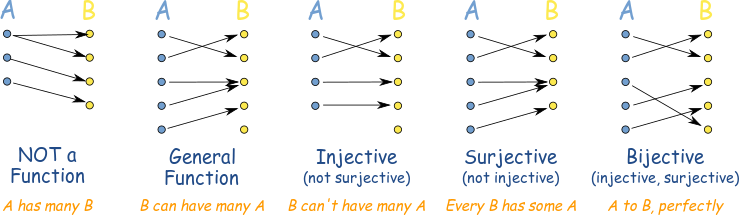
\includegraphics[width=\textwidth]{function-mapping.png}
    \caption{Injective, Surjective and Bijective}
    \label{fig:func}
\end{figure}


\section{Inequality}
There are 3 ways to solve inequality
\subsection{substitution}
Some example is $abc=4(a+b)$, find the minimum value of $a+b+c$.
\subsection{齐此化}
The logic is that you want to make the numerator and the denominator have the same power in the end. Then simplify it to something like $\frac{x}{y}+\frac{y}{x}$ and then use AM-GM.
\begin{itemize}
    \item Given that $x>0,y>0, x+2y=1$, what is the smallest value of $\frac{(x+1)(y+1)}{xy}$.
    \item If $x>0, y>0, x+2y=1$, what is the greatest value of $\frac{xy}{2x+y}$.
        
            
\end{document}
